\documentclass[12pt]{article}
\usepackage{amsmath}
\usepackage{graphicx}
\usepackage[export]{adjustbox}
\usepackage{geometry}

\begin{huge}
\title{Earthquake Magnitude vs. Space Weather Variables\\
\large Heatmaps sorted by Magnitude brackets}
\author{Zane van Campfort and Roman Avery}

\date{31/12/21}
\end{huge}
\setlength{\topmargin}{-1in}


\begin{document}
\maketitle
\begin{large}
All Space Weather variables that have been compared against magnitude in
previous documents are featured here.\newline


\centering Table of Contents:

\begin{description}
  \item Whole Dataset ---\null\hfill 2
\item Number of Entries: 32107
  \item Magnitude bracket (5.0-6.0)--- \null\hfill 5
\item Number of Entries: 25219
  \item Magnitude bracket (6.0-7.0) ---\null\hfill 8
\item Number of Entries: 6250
  \item Magnitude bracket (7.0-8.0) --- \null\hfill 11
\item Number of Entries: 632
  \item Magnitude bracket (8.0-9.0) --- \null\hfill 14
\item Number of Entries: 36
\end{description}
\end{large}

\graphicspath{{../plots/31_12/}}
\newgeometry{top=0.5in, left=0in}

\newpage

\begin{figure}
   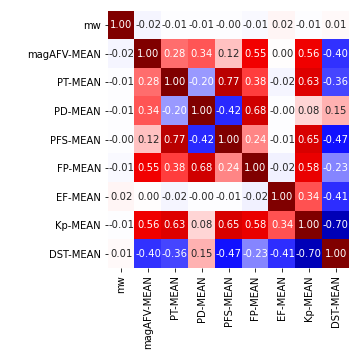
\includegraphics[width=0.57\textwidth]{all_mean_1.png}
   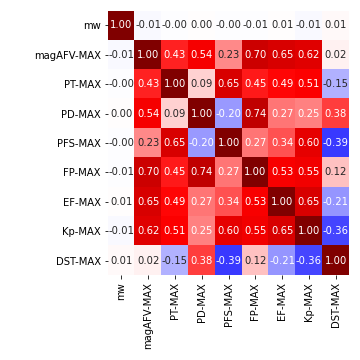
\includegraphics[width=0.57\textwidth]{all_max_1.png}
   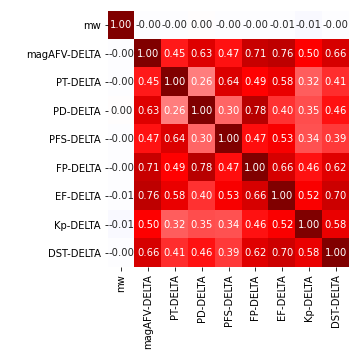
\includegraphics[width=0.57\textwidth]{all_delta_1.png}
   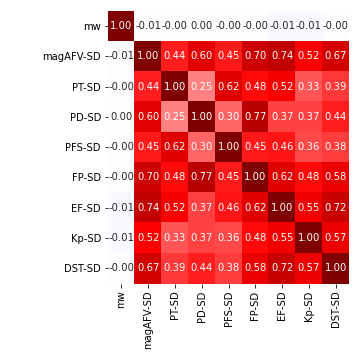
\includegraphics[width=0.57\textwidth]{all_sd_1.png}
\end{figure}

\newpage


\begin{figure}
   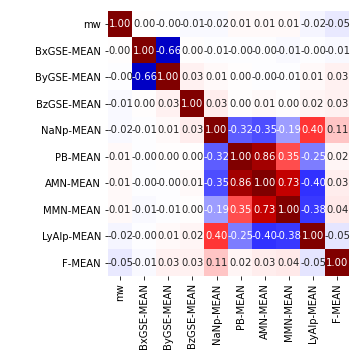
\includegraphics[width=0.57\textwidth]{all_mean_2.png}
   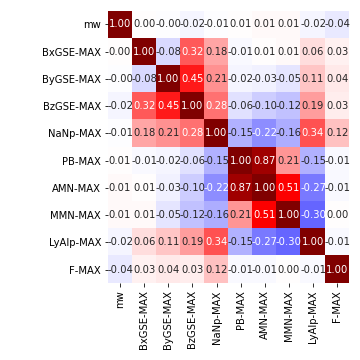
\includegraphics[width=0.57\textwidth]{all_max_2.png}
   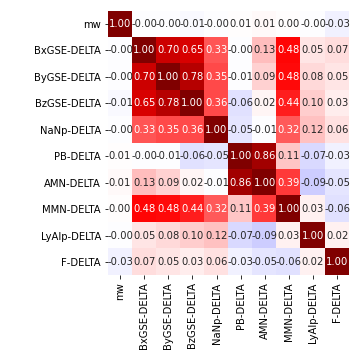
\includegraphics[width=0.57\textwidth]{all_delta_2.png}
   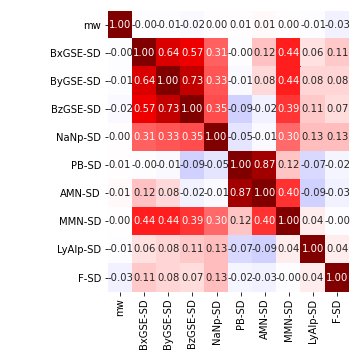
\includegraphics[width=0.57\textwidth]{all_sd_2.png}
\end{figure}

\newpage


\begin{figure}
   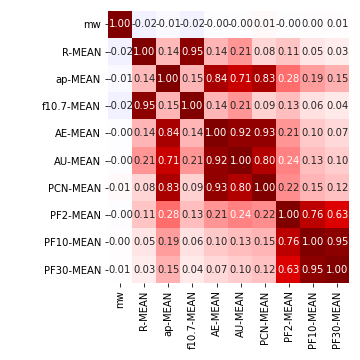
\includegraphics[width=0.57\textwidth]{all_mean_3.png}
   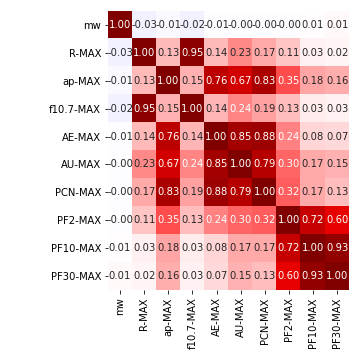
\includegraphics[width=0.57\textwidth]{all_max_3.png}
   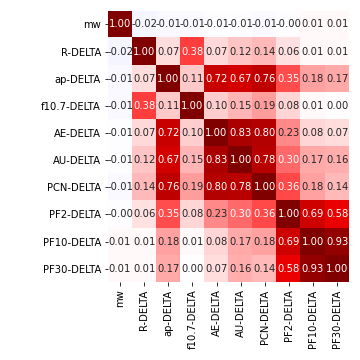
\includegraphics[width=0.57\textwidth]{all_delta_3.png}
   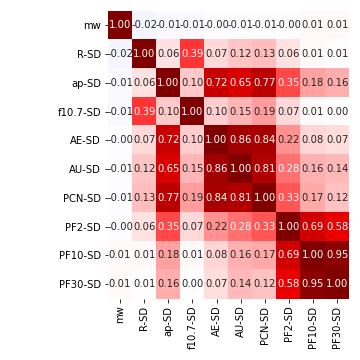
\includegraphics[width=0.57\textwidth]{all_sd_3.png}
\end{figure}

\newpage

\begin{figure}
   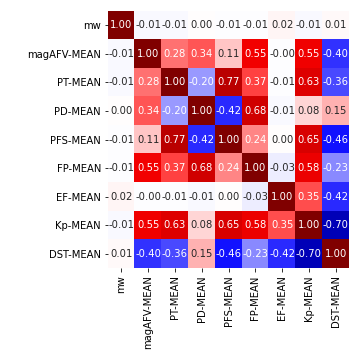
\includegraphics[width=0.57\textwidth]{five-six_mean_1.png}
   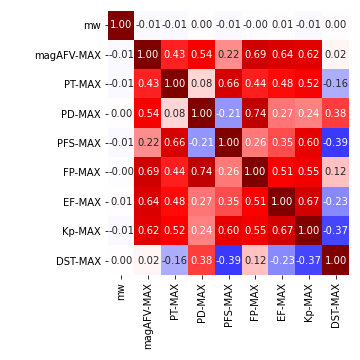
\includegraphics[width=0.57\textwidth]{five-six_max_1.png}
   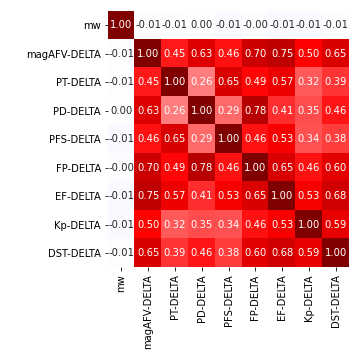
\includegraphics[width=0.57\textwidth]{five-six_delta_1.png}
   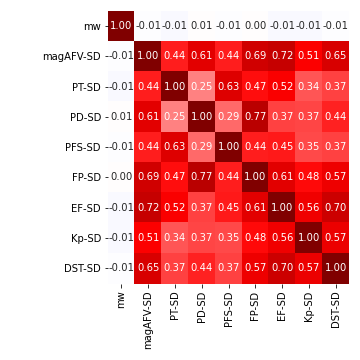
\includegraphics[width=0.57\textwidth]{five-six_sd_1.png}
\end{figure}

\newpage

\begin{figure}
   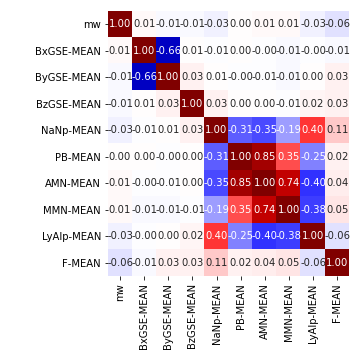
\includegraphics[width=0.57\textwidth]{five-six_mean_2.png}
   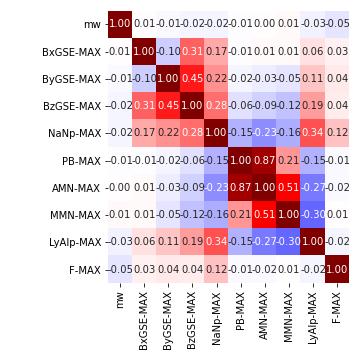
\includegraphics[width=0.57\textwidth]{five-six_max_2.png}
   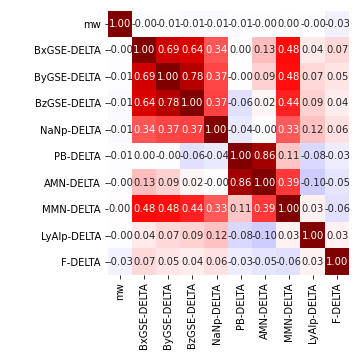
\includegraphics[width=0.57\textwidth]{five-six_delta_2.png}
   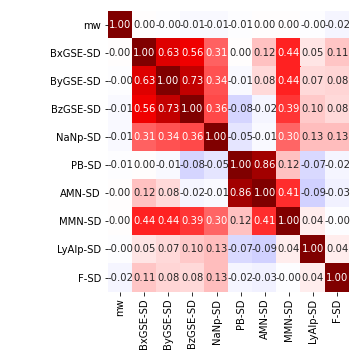
\includegraphics[width=0.57\textwidth]{five-six_sd_2.png}
\end{figure}

\newpage

\begin{figure}
   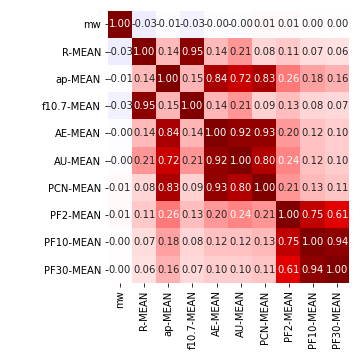
\includegraphics[width=0.57\textwidth]{five-six_mean_3.png}
   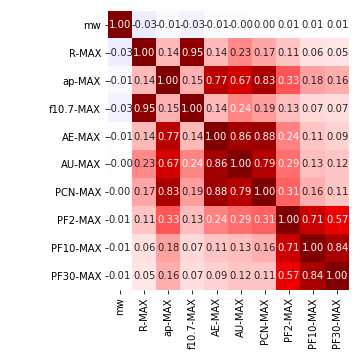
\includegraphics[width=0.57\textwidth]{five-six_max_3.png}
   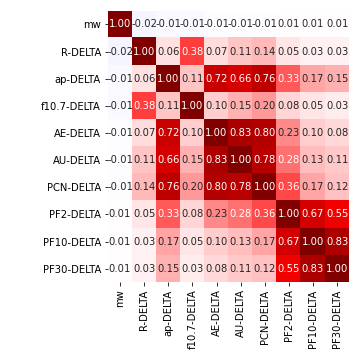
\includegraphics[width=0.57\textwidth]{five-six_delta_3.png}
   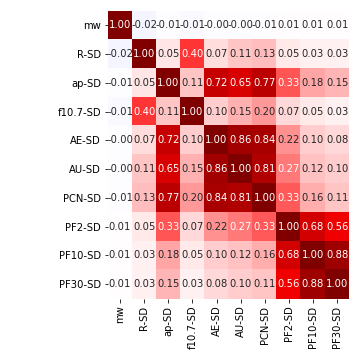
\includegraphics[width=0.57\textwidth]{five-six_sd_3.png}
\end{figure}

\newpage

\begin{figure}
   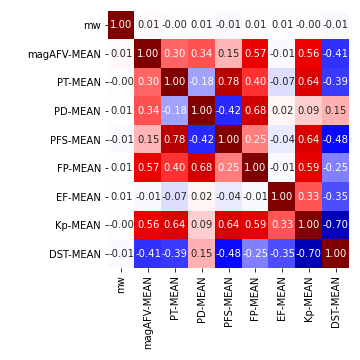
\includegraphics[width=0.57\textwidth]{six-seven_mean_1.png}
   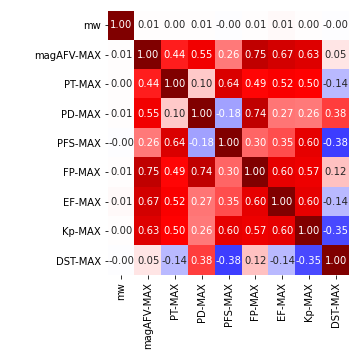
\includegraphics[width=0.57\textwidth]{six-seven_max_1.png}
   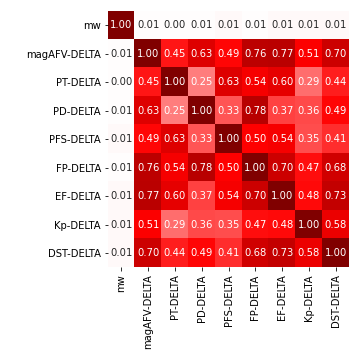
\includegraphics[width=0.57\textwidth]{six-seven_delta_1.png}
   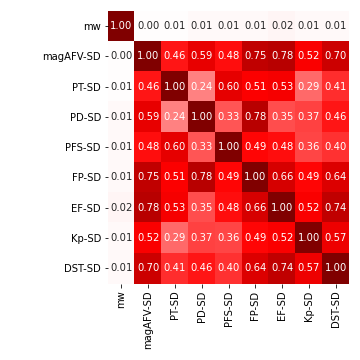
\includegraphics[width=0.57\textwidth]{six-seven_sd_1.png}
\end{figure}

\newpage

\begin{figure}
   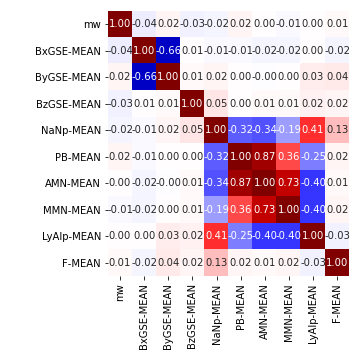
\includegraphics[width=0.57\textwidth]{six-seven_mean_2.png}
   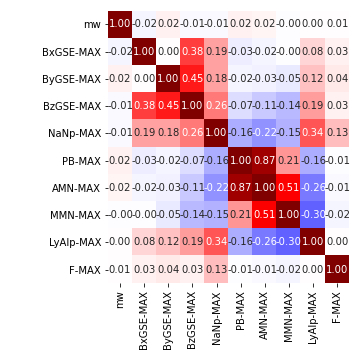
\includegraphics[width=0.57\textwidth]{six-seven_max_2.png}
   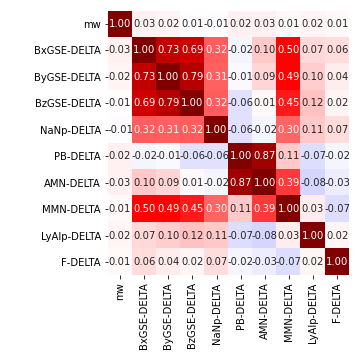
\includegraphics[width=0.57\textwidth]{six-seven_delta_2.png}
   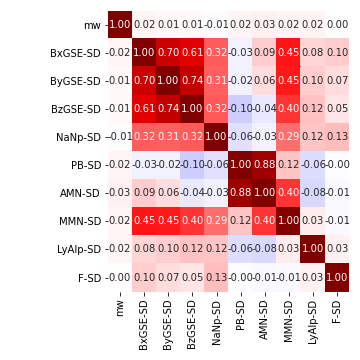
\includegraphics[width=0.57\textwidth]{six-seven_sd_2.png}
\end{figure}

\newpage

\begin{figure}
   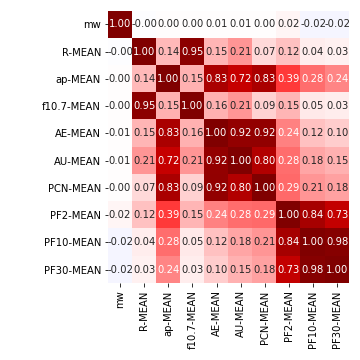
\includegraphics[width=0.57\textwidth]{six-seven_mean_3.png}
   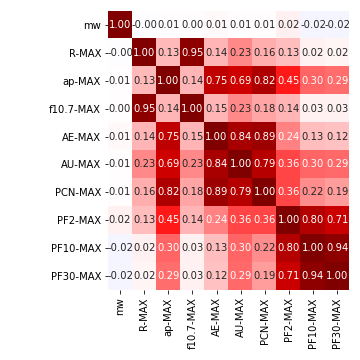
\includegraphics[width=0.57\textwidth]{six-seven_max_3.png}
   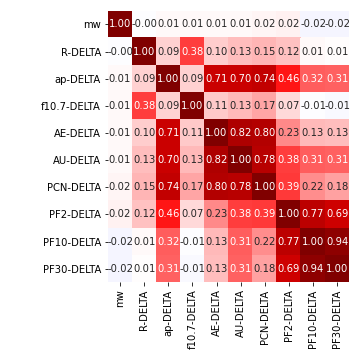
\includegraphics[width=0.57\textwidth]{six-seven_delta_3.png}
   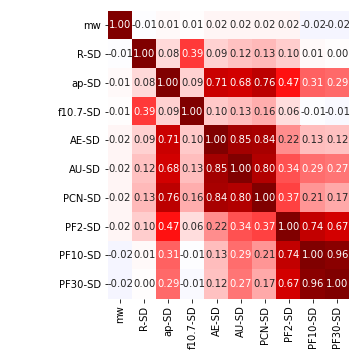
\includegraphics[width=0.57\textwidth]{six-seven_sd_3.png}
\end{figure}

\newpage

\begin{figure}
   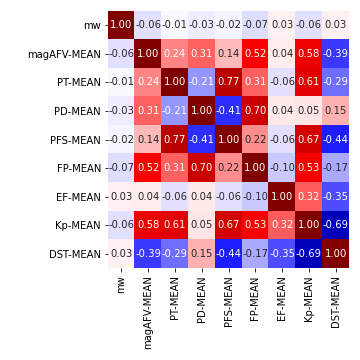
\includegraphics[width=0.57\textwidth]{seven-eight_mean_1.png}
   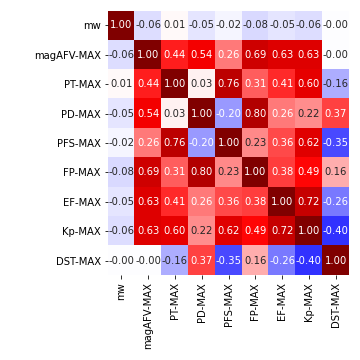
\includegraphics[width=0.57\textwidth]{seven-eight_max_1.png}
   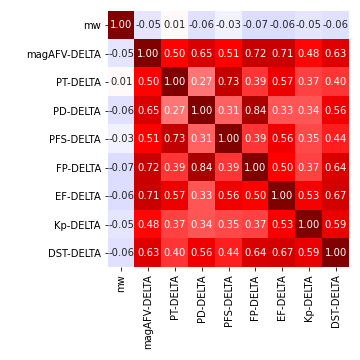
\includegraphics[width=0.57\textwidth]{seven-eight_delta_1.png}
   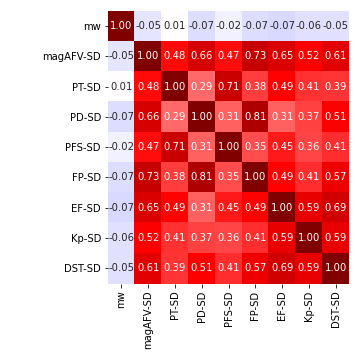
\includegraphics[width=0.57\textwidth]{seven-eight_sd_1.png}
\end{figure}

\newpage

\begin{figure}
   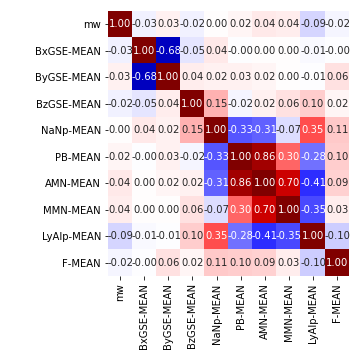
\includegraphics[width=0.57\textwidth]{seven-eight_mean_2.png}
   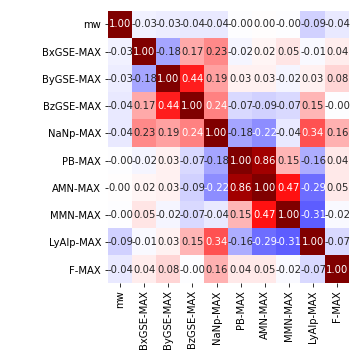
\includegraphics[width=0.57\textwidth]{seven-eight_max_2.png}
   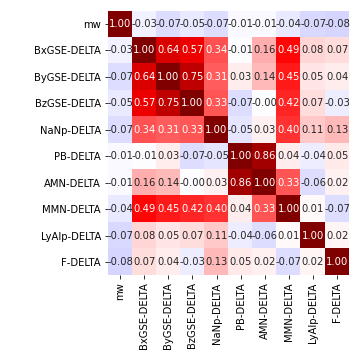
\includegraphics[width=0.57\textwidth]{seven-eight_delta_2.png}
   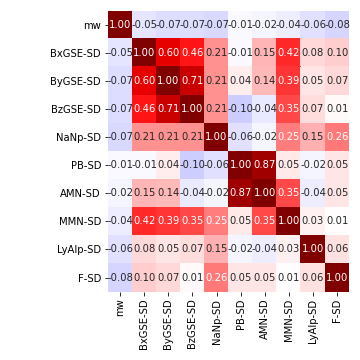
\includegraphics[width=0.57\textwidth]{seven-eight_sd_2.png}
\end{figure}

\newpage

\begin{figure}
   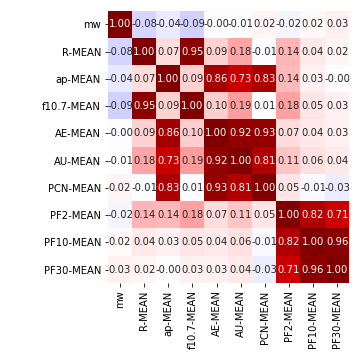
\includegraphics[width=0.57\textwidth]{seven-eight_mean_3.png}
   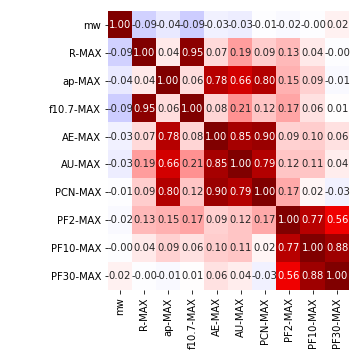
\includegraphics[width=0.57\textwidth]{seven-eight_max_3.png}
   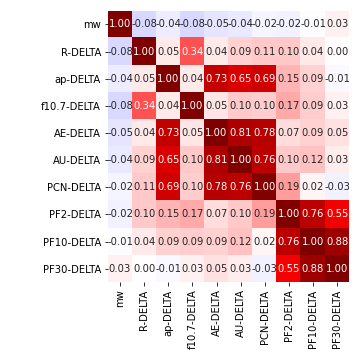
\includegraphics[width=0.57\textwidth]{seven-eight_delta_3.png}
   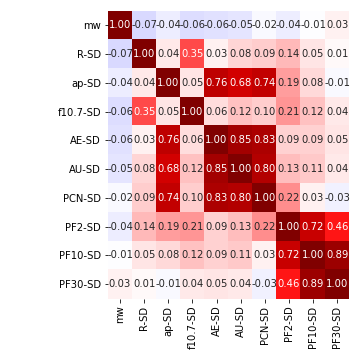
\includegraphics[width=0.57\textwidth]{seven-eight_sd_3.png}
\end{figure}

\newpage

\begin{figure}
   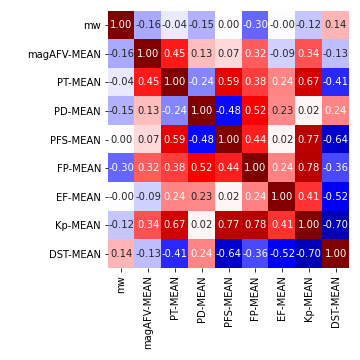
\includegraphics[width=0.57\textwidth]{eight-nine_mean_1.png}
   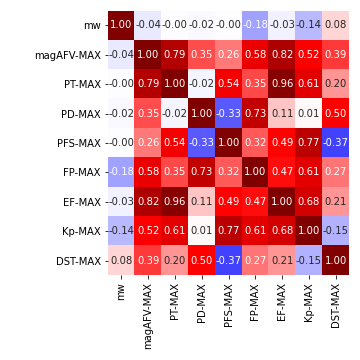
\includegraphics[width=0.57\textwidth]{eight-nine_max_1.png}
   \includegraphics[width=0.57\textwidth]{eight-nine_delta_1.png}
   \includegraphics[width=0.57\textwidth]{eight-nine_sd_1.png}
\end{figure}

\newpage

\begin{figure}
   \includegraphics[width=0.57\textwidth]{eight-nine_mean_2.png}
   \includegraphics[width=0.57\textwidth]{eight-nine_max_2.png}
   \includegraphics[width=0.57\textwidth]{eight-nine_delta_2.png}
   \includegraphics[width=0.57\textwidth]{eight-nine_sd_2.png}
\end{figure}

\newpage

\begin{figure}
   \includegraphics[width=0.57\textwidth]{eight-nine_mean_3.png}
   \includegraphics[width=0.57\textwidth]{eight-nine_max_3.png}
   \includegraphics[width=0.57\textwidth]{eight-nine_delta_3.png}
   \includegraphics[width=0.57\textwidth]{eight-nine_sd_3.png}
\end{figure}

\newpage



\end{document}